\documentclass{article}
% \usepackage{svg}
\usepackage{graphicx}
\usepackage{hyperref}
\usepackage[T1]{fontenc}
\usepackage{listings}
\usepackage{float}
\usepackage{xcolor}
\usepackage{amsmath}
\usepackage[margin=3cm]{geometry}
\usepackage{float}
\usepackage{tikz}
\usetikzlibrary{positioning, shapes.geometric, calc}
\graphicspath{{images/}{img/}}

\lstset{
	language=Python,
	basicstyle=\footnotesize\ttfamily,
	keywordstyle=\color{blue},
	commentstyle=\color{gray},
	stringstyle=\color{orange},
	breaklines=true,
	frame=lines,
	numbers=left,
	numberstyle=\tiny\color{gray}
}

\title{Speech Module - Technical Documentation}
\author{Mateusz Block, Lucjan Butko, Adam Macko}
\date{March 2026}

\begin{document}
	
	\maketitle
	\tableofcontents
	\newpage
	
	\section{Project Overview and Purpose}
	The main goal of the speech module, developed as part of the "humanoid-head" project, is to enable the robot to conduct natural and meaningful conversations with humans. Our team's task is to ensure that the machine not only reacts to rigid commands but can also respond fluently and logically to questions, mimicking a real conversation.
	
	The assistant was designed with the students of the Gdańsk University of Technology in mind. Its practical applications within this interaction include:
	\begin{itemize}
		\item Providing precise navigation directions, making it easier to reach specific rooms in university buildings (such as EA or NE).
		\item Providing up-to-date information about weather conditions.
		\item Engaging in casual conversations on general topics, using artificial intelligence to generate natural-sounding responses.
	\end{itemize}
	
	\section{System Architecture}
	The system is designed as a continuous loop that runs until it is stopped manually. It uses a pipeline structure with three main steps:
	\begin{itemize}
		\item \textbf{Speech-to-Text (STT):} The system uses a microphone to listen to the user. It records the sound and uses the Whisper AI model (the "small" version) to change the user's voice into text.
		\item \textbf{Intent Detection and Processing (LLM):} After getting the text, the system checks what the user wants using the \texttt{IntentDetector}.
		\begin{itemize}
			\item If the user asks about the weather ("POGODA") or university classes ("PG"), the system uses specific logic to find this data.
			\item For all other questions, it sends the text to a Large Language Model. The project uses the Ollama framework with the "gemma3:4b" model, connected through the LangChain library. The model gets a special prompt with a database of rooms and weather data to know how to answer correctly.
		\end{itemize}
		\item \textbf{Text-to-Speech (TTS):} When the text answer is ready, the system uses the \texttt{pyttsx3} library to read it out loud.
	\end{itemize}
	
	\section{Environment and Dependencies}
	
	\subsection{Required Libraries}
	The project relies on a variety of Python libraries for audio processing, web scraping, system integration, and data manipulation. The key dependencies are described below:
	
	\begin{itemize}
		\item \textbf{BeautifulSoup4} (\texttt{beautifulsoup4}): Used for parsing HTML documents. It is utilized to scrape information and extract staff details from the university's websites.
		\item \textbf{LangChain} (\texttt{langchain-core}, \texttt{langchain-ollama}): Manages the integration with local Large Language Models via Ollama and formats chat prompt templates.
		\item \textbf{PyAudio} (\texttt{pyaudio}): Provides Python bindings for PortAudio, essential for capturing live audio streams from the microphone.
		\item \textbf{Python Weather} (\texttt{python-weather}): An asynchronous library used to fetch current weather data and conditions.
		\item \textbf{pyttsx3} (\texttt{pyttsx3}): An offline Text-to-Speech (TTS) conversion library that allows the assistant to vocalize its responses to the user.
		\item \textbf{RapidFuzz} (\texttt{rapidfuzz}): A fast string matching library used for fuzzy search. It helps in matching spoken teacher names against the database, accommodating slight mispronunciations or transcription errors.
		\item \textbf{Requests} (\texttt{requests}): An HTTP library utilized to send requests to external university web pages for data scraping purposes.
		\item \textbf{SpeechRecognition} (\texttt{speechrecognition}): A wrapper library that facilitates capturing microphone input, detecting speech, and automatically adjusting for ambient noise levels.
	\end{itemize}
	
	\subsection{AI Models}
	The system implements the following artificial intelligence models and their associated frameworks to process user input, recognize entities, and generate appropriate responses:
	
	\begin{itemize}
		\item \textbf{Whisper ("small")}: A Speech-to-Text (STT) model developed by OpenAI (managed via the \texttt{openai-whisper} library), used to transcribe the audio captured from the user's microphone into text.
		\item \textbf{Gemma 3 (\texttt{gemma3:4b})}: A Large Language Model (LLM) served via Ollama. It is responsible for generating conversational responses for general queries when no specific predefined intent is detected.
		\item \textbf{GLiNER (\texttt{urchade/gliner\_multi-v2.1})}: A Named Entity Recognition (NER) model (implemented via the \texttt{gliner} library) utilized to extract specific information from the transcribed text. It identifies entities such as room codes and person names (using \texttt{room code} and \texttt{person} labels) to assist in university navigation queries.
		\item \textbf{spaCy (\texttt{pl\_core\_news\_sm})}: A pre-trained Polish language model operating within the \texttt{spacy} NLP library. It performs word lemmatization and tokenization to quickly and accurately match user queries against predefined intent keywords.
	\end{itemize}
	
	
	\section{Core Modules Implementation}
	
	\subsection{NLP Pipeline}
	The Natural Language Processing (NLP) pipeline acts as the central coordinator of the humanoid head's interaction system. Implemented primarily within the \texttt{NlpModel} class, it manages the continuous loop of listening, understanding, and responding to the user. The pipeline is composed of three main stages:
	
	\begin{enumerate}
		\item \textbf{Speech-to-Text (STT):} The pipeline continuously captures ambient audio via the microphone using the \texttt{SpeechRecognition} library, automatically adjusting for background noise. Once speech is detected, the audio is processed by the Whisper STT model to generate an accurate text transcription.
		\item \textbf{Intent Routing \& Processing:} The transcribed text is immediately forwarded to the Intent Detection module. This module classifies the user's query into specific operational branches:
		\begin{itemize}
			\item If a \textbf{Weather Intent} is detected, the system bypasses the LLM and directly queries the weather integration module to retrieve the current conditions.
			\item If a \textbf{PG (Politechnika Gdańska) Intent} is detected, the text is preprocessed and analyzed by the GLiNER model to extract entities such as room codes or personnel names, which are then passed to the university database modules.
			\item If \textbf{No Specific Intent} (General) is detected, the transcribed text is fed into the locally hosted Large Language Model (Gemma 3) via LangChain to generate a natural, conversational response.
		\end{itemize}
		\item \textbf{Text-to-Speech (TTS):} Regardless of which branch processes the query, the resulting answer is sent to the TTS module (\texttt{pyttsx3}) to be synthesized into audible speech, completing the interaction cycle.
	\end{enumerate}
	
	To better illustrate the data flow within the \texttt{NlpModel}, Figure \ref{fig:nlp_pipeline} presents the architectural diagram of the pipeline.
	
	\begin{figure}[H]
		\centering
		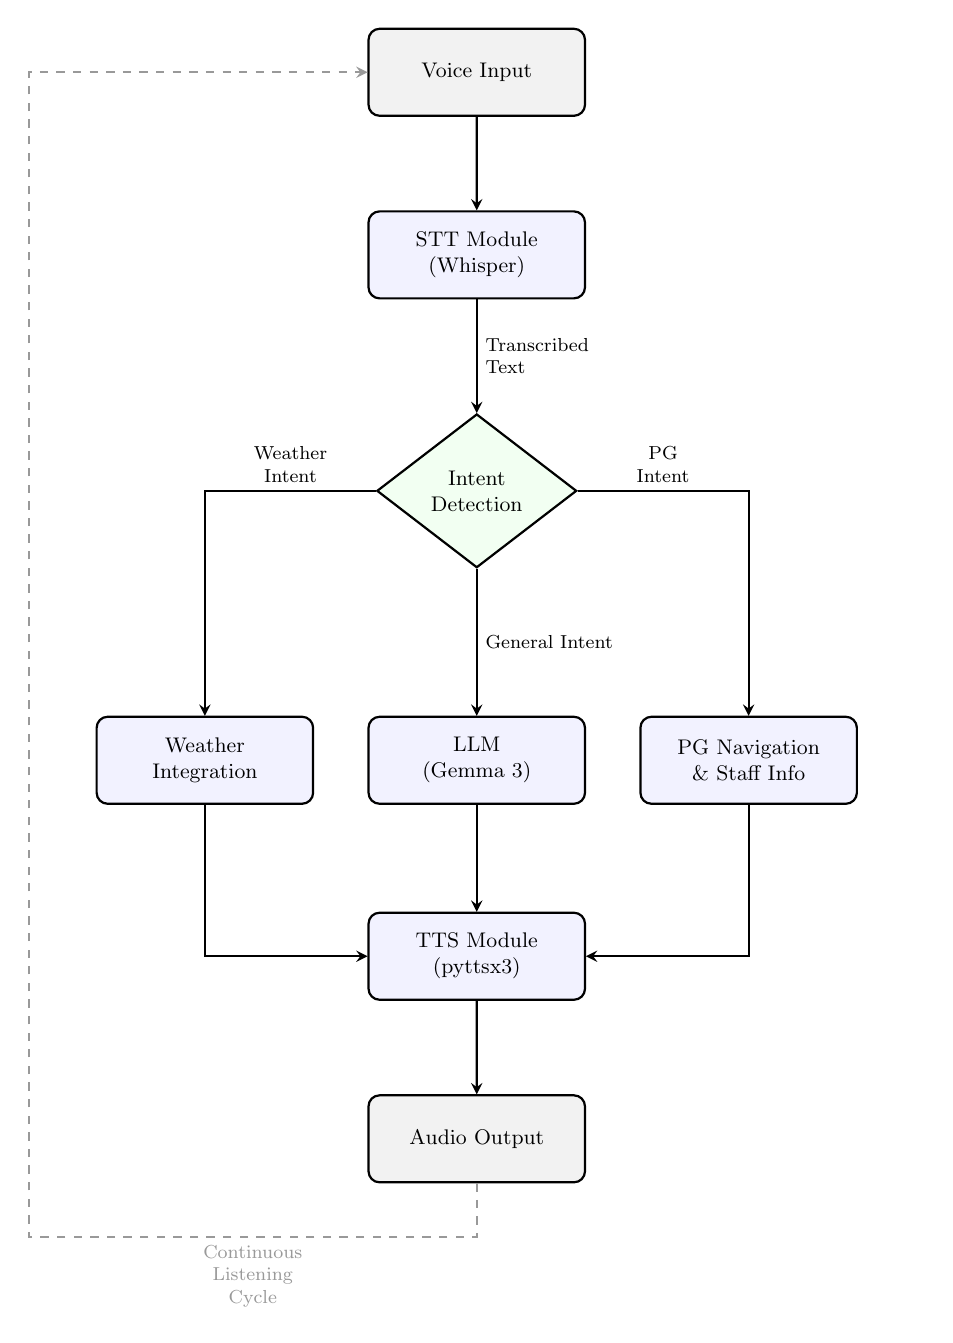
\begin{tikzpicture}[
			scale=0.85, transform shape,
			node distance=1.4cm and 0.8cm, 
			box/.style={rectangle, draw=black, thick, fill=blue!5, text width=3.0cm, align=center, minimum height=1.3cm, rounded corners, font=\small},
			decision/.style={diamond, draw=black, thick, fill=green!5, text width=2.2cm, align=center, inner sep=0pt, aspect=1.3, font=\small},
			arrow/.style={thick, ->, >=stealth},
			looparrow/.style={thick, ->, >=stealth, color=gray!80, dashed}
			]
			
			\node[box, fill=gray!10] (voice) {Voice Input};
			\node[box, below=of voice] (stt) {STT Module\\(Whisper)};
			\node[decision, below=of stt, yshift=-0.3cm] (intent) {Intent\\Detection};
			
			\node[box, below=of intent, yshift=-0.8cm] (llm) {LLM\\(Gemma 3)};
			
			\node[box, left=of llm] (weather) {Weather\\Integration};
			\node[box, right=of llm] (pg) {PG Navigation\\\& Staff Info};
			
			\node[box, below=of llm, yshift=-0.2cm] (tts) {TTS Module\\(pyttsx3)};
			\node[box, fill=gray!10, below=of tts] (audio) {Audio Output};
			
			\draw[arrow] (voice) -- (stt);
			\draw[arrow] (stt) -- (intent) node[midway, right, text width=2.2cm, align=left, font=\footnotesize] {Transcribed\\Text};
			\draw[arrow] (intent) -- (llm) node[midway, right, font=\footnotesize] {General Intent};
			\draw[arrow] (llm) -- (tts);
			\draw[arrow] (tts) -- (audio);
			
			\draw[arrow] (intent.west) -| (weather.north) node[near start, above, font=\footnotesize, align=center] {Weather\\Intent};
			\draw[arrow] (intent.east) -| (pg.north) node[near start, above, font=\footnotesize, align=center] {PG\\Intent};
			
			\draw[arrow] (weather.south) |- (tts.west);
			\draw[arrow] (pg.south) |- (tts.east);
			
			\coordinate (Lbottom) at ($(audio.south) + (0,-0.8cm)$);
			\coordinate (Lleft) at ($(weather.west) + (-1.0cm,0)$);
			
			\draw[looparrow] (audio.south) -- (Lbottom) -- (Lbottom -| Lleft)
			node[midway, below, align=center, font=\footnotesize] {Continuous\\Listening\\Cycle} -- (Lleft |- voice.west) -- (voice.west);
			
			\path ($(pg.east) + (1.0cm,0)$);
			
		\end{tikzpicture}
		\caption{NLP Pipeline Data Flow.}
		\label{fig:nlp_pipeline}
	\end{figure}
	
	\subsection{Intent Detection}
	The intent detection module is responsible for classifying the user's transcribed speech into one of the predefined categories, which determines how the query is routed within the NLP pipeline. This logic is encapsulated within the \texttt{IntentDetector} class.
	
	\subsubsection*{Initialization and Keyword Sets}
	The module uses the \texttt{spaCy} library along with the Polish language model (\texttt{pl\_core\_news\_sm}) to perform advanced text analysis. During initialization, it defines two primary sets of base words used for classification:
	\begin{itemize}
		\item \textbf{PG Keywords:} Terms related to the university, such as "sala", "wykład", "harmonogram", "profesor" and "dojść".
		\item \textbf{Weather Keywords:} Terms related to meteorological conditions, such as "pogoda", "temperatura", "deszcz" and "wiatr".
	\end{itemize}
	
	\subsubsection*{Operating Principle}
	The core classification is handled by the \texttt{detect\_intent()} method, which processes the input through the following steps:
	\begin{enumerate}
		\item \textbf{Text Preprocessing:} The raw input string is converted to lowercase and passed through the spaCy processing pipeline.
		\item \textbf{Lemmatization and Filtering:} The module iterates over the generated tokens, actively filtering out punctuation marks (\texttt{is\_punct}) and common Polish stop words (\texttt{is\_stop}). It extracts the base form (lemma) of each remaining token and stores them in a set for optimized searching.
		\item \textbf{Set Intersection and Classification:} The system uses logical set intersections to check for overlaps between the extracted lemmas and the predefined keyword sets. 
		\begin{itemize}
			\item If an intersection with the university keywords is found, it returns the \texttt{"PG"} intent.
			\item If an intersection with the weather keywords is found, it returns the \texttt{"POGODA"} intent.
			\item If there are no matches, the function returns \texttt{"OGOLNA"} intent (general intent), signaling the pipeline to process the query using the large language model.
		\end{itemize}
	\end{enumerate}
	
	\subsection{Weather Integration}
    To provide accurate, real-time meteorological data, the speech module incorporates a dedicated deterministic tool encapsulated within the \texttt{new\_weather.py} script. This module serves as a direct bridge to external meteorological APIs.
    
    The weather retrieval pipeline operates through the following sequence:
    \begin{itemize}
        \item \textbf{Data Retrieval:} The system sends an HTTP GET request to the Open-Meteo API. The query is hardcoded with the exact geographic coordinates of the city of Gdańsk (latitude 54.3523, longitude 18.6491) and requests specific metrics—primarily the current ambient temperature and the standard WMO (World Meteorological Organization) weather code.
        \item \textbf{WMO Code Mapping:} Raw numerical weather codes returned by the API are cross-referenced against a predefined local dictionary. This dictionary translates the numerical states directly into descriptive Polish phrases (e.g., "Bezchmurnie", "Lekki deszcz", "Burza").
        \item \textbf{Direct Prompt Generation:} The fetched weather description are automatically combined into a fully formed, natural-sounding Polish sentence ready for vocalization. 
    \end{itemize}
    
    When the \texttt{IntentDetector} identifies the \texttt{"POGODA"} (Weather) intent, the central execution pipeline completely bypasses the LLM and triggers this script. The generated weather string is routed instantly to the Text-to-Speech (TTS) engine.

	\subsection{Database Architecture}
To ensure deterministic, high-performance retrieval of spatial and personnel data, the speech module decouples its operational knowledge from the core Large Language Model. Instead of relying on the parametric memory of the LLM—which is prone to hallucinations and temporal degradation—a structured data storage layer was engineered. This layer consists of specialized databases formatted in JSON. The choice of JSON provides a lightweight, readable, and highly structured schema that allows for seamless parsing, and straightforward keyword-based queries within the Python environment.

The storage layer is fundamentally divided into three distinct database files, each handling a specific semantic domain of the Faculty of Electronics, Telecommunications and Informatics (WETI):

\begin{itemize}
    \item \textbf{Room Navigation Database (\texttt{room\_directions.json})}: 
    This database establishes a structural mapping of numbered classrooms, laboratories, and administrative offices across the EA (WETI A) and NE (WETI B) buildings. Each entry is keyed by a unique identifier combining the building code and the room number. The underlying payload contains explicit, step-by-step human-readable navigational routing instructions. These directions are written from the perspective of a user.
    
    \item \textbf{Specialized Locations Database (\texttt{db\_specialrooms.json})}: 
    To handle facility locations that do not follow standard room-numbering conventions, a separate semantic database was implemented. This file stores routing directions to these facilities.
    
    \item \textbf{Academic Staff Database (\texttt{teachers\_info.json})}: 
    This repository acts as the primary registry for the faculty's human resources and academic staff. Every entry is mapped to the full name of the researcher or administrative employee. The schema encapsulates critical metadata fields, including formal academic titles, the formally assigned institutional department (chair), and the office (building and room number). In instances where a staff member does not have a permanently assigned public office, the room schema dynamically defaults to a standardized \texttt{"Brak"} token, preventing the system from outputting corrupted or missing structural data.
\end{itemize}

By isolating these data vectors into a flat, well-indexed JSON topography, the system achieves sub-millisecond data lookup times. This architecture guarantees that any navigational or informational response delivered is grounded strictly in verified data.
	
\subsection{Algorithms for Database Retrieval}
The core operational logic of the retrieval layer is driven by a suite of dedicated Python scripts designed specifically to query the structured JSON databases. They receive data that has already been extracted into a concrete, specific format by the preceding GLiNER sequence. The scripts process these inputs to return the corresponding, factual data.
\begin{itemize}
    \item \textbf{Room Localization (\texttt{find\_room.py})}: 
    This script is tasked with querying the room navigation database. Before a database query is executed, the raw string extracted from user input is subjected to a normalization pipeline that eliminates whitespace discrepancies, converts characters to uppercase, and applies regular expressions to standardize the string. If the normalized key exists within \texttt{room\_directions.json}, the script directly returns the explicit human-readable navigation payload.
    
    \item \textbf{Specialized Locations Retrieval (\texttt{find\_aud.py})}: 
    Operating analogously to the room localization script, this component handles queries regarding facility areas that do not conform to standard, sequential room numbers (such as auditoriums, libraries, or cafeterias). By mirroring the parsing structure of the room lookup but targeting \texttt{db\_specialrooms.json}, it isolates semantic location queries and rapidly routes the corresponding floor parameters and customized directions.
    
    \item \textbf{Academic Staff Query and Coordination Pipeline (\texttt{find\_teacher.py})}: 
    This script manages the retrieval of personnel data from \texttt{teachers\_info.json}. When a staff identity is queried, the script executes a fuzzy string matching search across the database keys. Upon finding a valid entry, it extracts the staff member's profile metadata and returns their assigned coordinates (building prefix and office number). To ensure seamless operational continuity, these coordinates are then programmatically passed into the \texttt{find\_room.py} pipeline, which automatically resolves and streams the explicit routing directions for that specific office to the user.
\end{itemize}

\subsubsection*{Interactive Fallback for Ambiguous Queries}
To further improve the reliability of the staff retrieval algorithm, an interactive fallback mechanism was introduced. When the fuzzy matching algorithm identifies multiple potential candidates with a confidence score falling between the strict top threshold and the baseline threshold, the system actively engages the user. It presents the top three most probable faculty members and asks the user to select the correct one by speaking a corresponding number (0, 1, or 2). This interactive disambiguation ensures accurate guidance even when the user's initial query is vague or the STT transcription is imprecise.
	
	\subsection{Text-to-Speech and Asynchronous Streaming}
	To improve the naturalness and responsiveness of the conversation, the system transitioned from the traditional \texttt{pyttsx3} library to \textbf{PiperTTS}, utilizing a high-quality Polish acoustic model in \texttt{.onnx} format. This upgrade significantly enhances the voice quality and makes the humanoid sound much more lifelike.
	
	Furthermore, to minimize the perceived latency, the TTS module implements asynchronous streaming. Instead of waiting for the Large Language Model to generate the entire response, the system utilizes Python threading and queues. A dedicated background thread monitors the LLM's output character by character. Upon detecting punctuation marks (indicating the end of a phrase or sentence), it immediately chunks the text and sends it to the PiperTTS engine. This architecture allows the humanoid head to begin speaking almost instantly while the LLM continues generating the rest of the response in parallel.
	
	\subsection{Identity and Emotion Management}
	A key advancement in creating a compelling human-robot interaction is the ability to recognize the user's identity and emotional state. The system features a dedicated \texttt{get\_new\_user\_name} routine, where the assistant introduces itself and asks for the user's name if they are unrecognized. The transcribed spoken name is then matched against a local database of Polish names (\texttt{imiona\_polskie.txt}) using fuzzy matching via the \texttt{rapidfuzz} library. This ensures robust name recognition even if the Speech-to-Text model slightly misinterprets the pronunciation.
	
	In addition to voice interactions, the speech module integrates a local API server built with the \textbf{Flask} framework (exposing the \texttt{/api/data} endpoint). This endpoint allows external systems (such as a vision or facial recognition module) to continuously update the current user's identity and detected emotion. The emotions are mapped through an \texttt{EMOTION\_PL\_MAP} to Polish equivalents (e.g., mapping "Happy" to "radość"). This state is subsequently synchronized with the main Raspberry Pi controller via HTTP requests to maintain a coherent behavioral state across all of the robot's subsystems.
	
	\section{Prompt Engineering}
	\subsection{System Prompt}
	The system prompt establishes the assistant as a helpful guide for students of the Gdańsk University of Technology. 
	
	If the intent module detects a general conversational intent rather than a specific command, the system uses this prompt to guide the Large Language Model. The user's transcribed query is simply injected into the \texttt{\{question\}} placeholder, allowing the AI to generate a natural, contextual response.
	\subsection{Deterministic Retrieval and Tool Calling}
	During the initial development phases, the implementation of a Retrieval-Augmented Generation (RAG) architecture was considered. Ultimately, the RAG approach was abandoned in favor of a deterministic "Tool Calling" architecture. 
	
	When the system detects a specific, university-related intent, it bypasses the LLM's generative capabilities. Instead, the text is processed by the \textbf{GLiNER} model (for Named Entity Recognition) to extract key parameters, which then triggers dedicated Python scripts to fetch hardcoded, verified data. The two primary retrieval tools used in this process are:
	
	\begin{itemize}
		\item \textbf{\texttt{find\_room.py} (Exact Match Retrieval):} This script is executed when the GLiNER model extracts a \texttt{room code} entity. It takes a formatted input string, splits it into building and room components using a comma delimiter, and performs a strict exact-match search within the \texttt{room\_directions.json} database. If a match is found, it directly returns the precise, step-by-step navigation instructions.
		
		\item \textbf{\texttt{find\_teacher.py} (Fuzzy Match Retrieval):} This script is invoked when a \texttt{person} entity is detected by GLiNER. Because Speech-to-Text models often mistranscribe proper nouns and surnames, an exact match approach would frequently fail. To solve this, the script utilizes the \texttt{rapidfuzz} library to calculate a string similarity score against the \texttt{teachers\_info.json} database. If the match score meets or exceeds the defined threshold of 50\%, the system assumes a successful identification and retrieves the professor's assigned office location.
	\end{itemize}
	
	By employing these retrieval scripts as external tools, the system guarantees factual accuracy in its navigational responses and significantly reduces latency, completely mitigating the risk of LLM hallucinations.
	
	\subsection{Conversation History and Context Buffer}
	To support multi-turn conversations and maintain context over time, a conversation history buffer was introduced. Implemented using a double-ended queue (\texttt{collections.deque}), it retains a fixed number of recent interactions, defined by the \texttt{CONVERSATION\_BUFFER\_LEN} constant. When the buffer reaches its capacity, the oldest exchanges are automatically discarded to keep the LLM's context window optimized and prevent memory overflow.
	
	The system prompt has been enhanced to inject dynamic variables directly into the template before invoking the LLM. The pipeline provides the structured \texttt{\{history\}} of the conversation, the current user's \texttt{\{name\}}, and their detected \texttt{\{emotion\}}. This context injection allows the Gemma model to highly personalize its responses—for instance, by addressing the user by their name or adjusting its conversational tone based on whether the user is currently happy, sad, or neutral.
	
\end{document}
